\documentclass[amssymb,twocolumn,pra,10pt,aps]{revtex4-1}
\usepackage{mathptmx,amsmath,amsthm,hyperref}
\usepackage{tikz}

\newtheorem{lemma}{Lemma}
\newtheorem{cor}[lemma]{Corollary}
\newtheorem*{lemma*}{Lemma}
\newcommand{\FF}{\mathbb{F}}
\newcommand{\QQ}{\mathbb{Q}}
\newcommand{\RR}{\mathbb{R}}
\newcommand{\CC}{\mathbb{C}}
\newcommand{\ZZ}{\mathbb{Z}}

\begin{document}

\title{Solutions to the 86th William Lowell Putnam Mathematical Competition \\
    Saturday, December 6, 2025}
\author{Manjul Bhargava, Kiran Kedlaya, and Lenny Ng}
\noaffiliation
\maketitle

\begin{itemize}
\item[A1]
For each $k\geq 0$, the numbers $2m_k+1$ and $2n_k+1$ are odd and hence their greatest common factor $d_k$ must be odd. For an integer $r$, let $\mathrm{Odd}(r)$ denote the largest odd factor of $r$. Then note that
\begin{align*}
\mathrm{Odd}(m_{k+1}-n_{k+1}) &= \mathrm{Odd}\left(\frac{2m_k+1}{d_k}-\frac{2n_k+1}{d_k}\right) \\
  &= \mathrm{Odd}\left(\frac{m_k-n_k}{d_k}\right) \leq \mathrm{Odd}(m_k-n_k),
\end{align*}
with equality if and only if $d_k=1$.
Thus $\mathrm{Odd}(m_k-n_k)$ is a nonincreasing sequence of positive integers, decreasing only when $d_k>1$. Hence the sequence $\mathrm{Odd}(m_k-n_k)$ must stabilize once $k$ is greater than some $K$, implying that $d_k=1$ for $k>K$; that is, $2m_k+1$ and $2n_k+1$ are relatively prime for all $k>K$, as desired.


\item[A2]
The answer is $a=1/\pi$ and $b=4/\pi^2$. 

\noindent
\textbf{First solution.}
It suffices to restrict to $x \in [0,\pi/2]$ rather than $x \in [0,\pi]$ since the given inequalities are unchanged if we replace $x$ by $\pi-x$. Define the function 
\[
f(x) = \frac{\sin x}{x(\pi-x)},
\]
and note that $f$
is differentiable on $(0,\pi/2]$ and can be extended continuously to $x=0$ by setting $f(0) = 1/\pi$.
In particular, if $a$ and $b$ satisfy the desired condition, then $a \leq 1/\pi$ and
and $b \geq f(\pi/2) = 4/\pi^2$; it thus suffices to check that $a = 1/\pi$ and $b = 4/\pi^2$ satisfy the condition.

 We compute that $f'(x) = \frac{g(x)}{x^2(\pi-x)^2}$ for
 \[
 g(x) = x(\pi-x)\cos x-(\pi-2x)\sin x.
\]

We claim that $g(x) > 0$ for all $x \in (0,\pi/2)$. Indeed, note that $g(0)=g(\pi/2)=0$ and
\[
g'(x) = (x^2-\pi x+2)(\sin x).
\]
Noting that the quadratic $x^2-\pi x+2$ is positive at $x=0$ and negative at $x=\pi/2$, we see that it has a root $r \in (0,\pi/2)$,
 is positive before that root, and is negative after that root. That is, $g'(x)>0$ for $x \in (0,r)$ and $g'(x)<0$ for $x \in (r,\pi/2)$. If some $x_0 \in (0,\pi/2)$ satisfied $g(x_0) \leq 0$, then we would have both $x_0>r$ since $g$ is increasing in $(0,r)$
 and $g(0)=0$, and $x_0<r$ since $g$ is decreasing in $(r,\pi/2)$ and $g(\pi/2)=0$, contradiction. This proves the claim.

Since $f'(x)>0$ on $(0,\pi/2)$, it follows that $f(x)$ is strictly increasing on $[0,\pi/2]$ and hence achieves a minimum at $f(0) = 1/\pi$ and a maximum at $f(\pi/2) = 4/\pi^2$. Consequently, $a=1/\pi$ and $b=4/\pi^2$ satisfy the desired condition as claimed.

\noindent
\textbf{Second solution.}
As in the first solution, we reduce to checking that $a=1/\pi$ and $b = 4/\pi^2$ satisfy the given inequality for $x \in [0, \pi/2]$.
For the lower bound, we use the fact that for $x \in [0, \pi/2]$,
\[
\sin x \geq x - \frac{1}{6} x^3
\]
(by either Taylor's theorem with remainder or the alternating series test) and the fact that $\pi^2 < 12$ to obtain
\begin{align*}
\sin x - \frac{1}{\pi} x(\pi - x) &\geq x - \frac{1}{6} x^3 - \frac{1}{\pi}x(\pi-x) \\
&= x^2 \left( \frac{1}{\pi} - \frac{x}{6} \right) \\
&\geq x^2 \left( \frac{1}{\pi} - \frac{\pi}{12} \right) \geq 0.
\end{align*}
For the upper bound, set
\[
f(x) = \frac{4}{\pi} x(\pi-x) - \sin x,
\]
so that $f(0) = f(\pi/2) = 0$, then compute that
\[
f'(x) = \frac{4}{\pi} - \frac{8}{\pi^2} x - \cos x, \quad
f''(x) = -\frac{8}{\pi^2} + \sin x.
\]
Since $\pi^2 > 8$, $f''(x)$ has exactly one root in $[0, \pi/2]$ and $f''(\pi/2) > 0$.
Since $f'(0)> 0$, $f'(\pi/2) = 0$, and $f''(\pi/2) > 0$, 
by Rolle's theorem $f'$ has exactly one root $r$ in $[0, \pi/2)$,
at which $f''$ is negative. Consequently, the absolute minimum of $f$ occurs as the endpoints,
proving the claim.

\noindent
\textbf{Third solution.} (by Catalin Zara)
As in the first solution, we reduce to checking that $a=1/\pi$ and $b = 4/\pi^2$ satisfy the given inequality for $x \in [0, \pi/2]$. For the lower bound, note that
$\cos \,t$ is concave on $[0, \pi/2]$, so $\cos \,t \geq 1 - (2/\pi)t$ and hence
\[
\sin x = \int_0^x \cos t\,dt \geq \int_0^x \left(1 - \frac{2}{\pi} t\right)\,dt  = \frac{1}{\pi}x(\pi-x).
\]
For the upper bound, note that $\sin \,t$ is concave on $[0, \pi/4]$, so $\sin \,t \geq (2\sqrt{2}/\pi)t$
and so
\begin{align*}
\sin x &= \cos \left( \frac{\pi}{2} - x \right)= 1 - 2 \sin^2 \left( \frac{\pi}{4} - \frac{x}{2} \right) \\
&\leq 1 - \frac{16}{\pi^2} \left( \frac{\pi}{4} - \frac{x}{2} \right)^2 = \frac{4}{\pi^2} x(\pi-x).
\end{align*}


\item[A3]
Bob has a winning strategy for all $n \geq 1$.

Consider the graph $G$ with vertices $\{0,1,2\}^n \setminus \{(0,\dots,0)\}$ with an edge between any two strings that differ by adding or subtracting 1 in a single position. A \emph{perfect matching} of $G$ consists of a collection $P$ of edges of $G$ which contain each vertex exactly once. Each perfect matching $G$ leads to a winning strategy for Bob: if Alice's last move was to vertex $v$, Bob moves to the vertex $w$ such that $\{v,w\} \in P$. This maintains the condition that before every move by Alice, the unused vertices still admit a perfect matching contained in $P$; consequently, Bob's next move is always legal.

It thus suffices to exhibit a perfect matching on $G$; there are many ways to do this. For example,
for each vertex $v$, find the first nonzero coordinate of $v$, let $w$ be the result of interchanging $1$ with $2$ in that position, and include $\{(v,w)\}$ in $P$; since running this process with $w$ leads back to $v$, we see that $P$ is a perfect matching. (For this matching, Bob's strategy is to  always change the first nonzero digit from 1 to 2 or \emph{vice versa}.)

\item[A4]
The minimal value of $k$ is 3.

We first produce a suitable sequence of matrices with $k=3$;
for this, we conflate $3 \times 3$ matrices with the linear transformations on $\RR^3$ that they define.
Choose unit vectors $\mathbf{v}_1,\dots,\mathbf{v}_{2025} \in \RR^3$
in general position (no two collinear, no three coplanar),
interpreting the indices cyclically so that $\mathbf{v}_i = \mathbf{v}_{2025+i}$.
Let $A_i$ be the unique linear transformation for which
\[
A_i(\mathbf{v}_i) = \mathbf{v}_i, \quad
A_i(\mathbf{v}_{i-1}) = A_i(\mathbf{v}_{i+1}) = 0.
\]
To check that $A_i$ commutes with $A_{i+1}$, note that the plane spanned by $\mathbf{v}_{i-1}$ and $\mathbf{v}_{i+1}$
intersects the plane spanned by $\mathbf{v}_i$ and $\mathbf{v}_{i+2}$ in a line; let $\mathbf{w}_i$ be a nonzero vector along this line. 
(Explicitly, we may take $\mathbf{w}_i = (\mathbf{v}_{i-1} \times \mathbf{v}_{i+1}) \times (\mathbf{v}_i \times \mathbf{v}_{i+2})$.)
Then $\mathbf{v}_i, \mathbf{v}_{i+1}, \mathbf{w}_i$ is a basis of $\RR^3$ with respect to which both $A_i$ and $A_{i+1}$ are diagonal, which implies that $A_i$ and $A_{i+1}$ commute.

To check that $A_i$ does not commute with $A_j$ when $j -i\not\equiv 0,1,-1 \pmod{2025}$,
note that any (complex) eigenvector of $A_i$ is either a scalar multiple of $\mathbf{v}_i$ or a linear combination of $\mathbf{v}_{i-1}$ and $\mathbf{v}_{i+1}$. In particular $\mathbf{v}_j$ is not an eigenvector of $A_i$, whereas
any matrix commuting with $A_j$ must admit $\mathbf{v}_j$ as an eigenvector.

We next show that no such sequence exists for $k=2$. 
Assume by way of contradiction that such a sequence exists. Then none of the $A_i$ can be a scalar matrix, as then it would commute with $A_{j}$ for all $j$. Also, no $A_i$ can have two distinct complex eigenvalues: any matrix commuting with $A_i$ would then be simultaneously diagonalizable with $A_i$, and any two such matrices commute with each other. Hence each $A_i$ has a unique real eigenvalue $\lambda_i$ and a unique eigenvector $\mathbf{v}_i$ up to scaling; we can replace each $A_i$ with $A_i - \lambda_i I$ (where $I$ denotes the $2 \times 2$ identity matrix) to reduce to the case where each $A_i$ is nilpotent. However, at this point $A_i$ can only commute with $A_{i+1}$ if $\mathbf{v}_i$ and $\mathbf{v}_{i+1}$ are parallel, which again implies that all of the matrices commute with each other.

\noindent
\textbf{Remark.}
A special case of this construction is to take $A_i := \mathbf{u}_i \mathbf{u}_i^T$ where the unit vectors $\mathbf{u}_i$ and $\mathbf{u}_j$ are orthogonal if and only if $|j-i| \in \{1,2024\}$.

\item[A5]
The sequences $s$ for which $f(s)$ are maximal are the alternating sequences
\[
((-1)^i \colon i=1,\dots,n-1), \quad
((-1)^{i+1} \colon i=1,\dots,n-1).
\]
For convenience we permit the case $n=1$, where the two sequences collapse to the empty sequence.

\noindent
\textbf{First solution.}
For a permutation $(a_1,\dots,a_n)$ of $\{1,2,\dots,n\}$, we refer to the unique sequence
$(s_1,\dots,s_{n-1}) \in \{\pm 1\}^{n-1}$ satisfying $s_i(a_{i+1}-a_i) > 0$ for all $i$
as the \emph{descent pattern} of $(a_1,\dots,a_n)$. In this language, $f(s)$ counts permutations with descent pattern $s$. 

For $s \in \{\pm 1\}^{n-1}, j \in \{1,\dots,n\}$, let $f(s,j)$ be the number of permutations
$(a_1,\dots,a_{n})$ with $a_{n} = j$ having descent pattern $s$, so that
\[
f(s) = \sum_{j=1}^n f(s,j).
\]
Writing $-s$ for the sequence $(-s_1,\dots,-s_{n-1})$, we have $f(s,j) = f(-s,n+1-j)$
on account of the bijection
\[
(a_1,\dots,a_n) \mapsto (n+1-a_1,\dots,n+1-a_n).
\]

Let $s_+ \in \{\pm 1\}^{n}$ be the sequence $s$ with $1$ appended.
We then have
\[
f(s_+, j) = \sum_{i=1}^{j-1} f(s, i) \qquad (j=1,\dots,n+1):
\]
a permutation $(a_1,\dots,a_n,j)$ has descent pattern $s_+$ if and only if $a_n \in \{1,\dots,j-1\}$
and the permutation obtained from $(a_1,\dots,a_n)$ by subtracting 1 from each entry greater than $j$ has descent pattern $s$. 
In particular,
\[
f(s_+, j) \leq f(s_+, j+1) \qquad (j=1,\dots,n).
\]
Moreover, $f(s_+, n+1) = f(s) > 0$.

Let $s_{++}, s_{+-} \in \{\pm 1\}^{n+1}$ be the sequence $s_+$ with $+1$ or $-1$ appended, respectively. By writing
\begin{align*}
f(s_{++},j) &= \sum_{i=1}^{j-1} f(s_+, i),\\
f(s_{+-},n+3-j) &= \sum_{i=1}^{j-1} f(s_+, n+2-j+i)
\end{align*}
(using sign symmetry for the second equality)
and noting that $f(s_+, i) \leq f(s_+, n+2-j+i)$, we deduce that
\[
f(s_{++}, j) \leq f(s_{+-}, n+3-j) \quad (j=1,\dots,n+2);
\]
moreover, the inequality is strict for $1 < j < n+2$.

Recursing forward, we deduce that for any sequence $s \in \{\pm 1\}^{n-1}$ and any $j \in \{1,\dots,n-1\}$
such that $s_{j-1} = s_j = 1$, the sequence $t \in \{\pm 1\}^{n-1}$ with
\[
t_i = \begin{cases} s_i & i < j \\
-s_i & i \geq j
\end{cases}
\]
satisfies $f(s) < f(t)$. Since there are only finitely many sequences in $\{\pm 1\}^{n-1}$, maximal sequences exist and cannot contain two consecutive equal entries; this proves the claim.

\noindent
\textbf{Remark.}
One can also reinterpret the proof of the inequality $f(s) \leq f(t)$ without recursion, by exhibiting an explicit injective map from the sequences with descent pattern $s$ to the sequences with descent pattern $t$.

\noindent
\textbf{Second solution.} (communicated by the Putnam graders)
For a sequence $s \in \{\pm 1\}^{n-1}$, define the set $P$ of \emph{peaks} of $s$ 
to contain those $i \in \{1,\dots,n\}$ such that $s_{i-1} = 1$ if $i > 1$ and $s_i = -1$ if $i < n$.
Define the set $V$ of \emph{valleys} of $s$ as the peaks of the negated sequence $-s$. Then
\begin{align*}
f(s)&=\sum_{i\in P}\binom{n-1}{i-1}f(s_1,\dots,s_{i-2})f(s_{i+1},\dots,s_n)\\
&=\sum_{i\in V}\binom{n-1}{i-1}f(s_1,\dots,s_{i-2})f(s_{i+1},\dots,s_{n-1}),
\end{align*}
so
\begin{align*}
2f(s)&=\sum_{i\in P\sqcup V}\binom{n-1}{i-1}f(s_1,\dots,s_{i-2})f(s_{i+1},\dots,s_n)\\
&\le\sum_{i=1}^{n}\binom{n-1}{i-1}f(s_1,\dots,s_{i-2})f(s_{i+1},\dots,s_n).
\end{align*}

Let $t_n$ be the alternating sequence $(1,-1,\dots)$ of length $n-1$ and define $E_n := f(t_{n-1}) = f(-t_{n-1})$; note that $2E_n=\sum_{i=1}^{n}\binom{n-1}{i-1}E_{i-1}E_{n-i}$.
We now induct on $n$ (again taking $n=1$ as the base case).
Suppose that $n \geq 2$ and, for any $s\ne\pm t_{k}$ of length $k\le n-2$, we have $f(s)<E_{k+1}$. 
Then for $s$ of length $n-1$,
\begin{align*}
2f(s) &\le\sum_{i=1}^{n}\binom{n-1}{i-1}f(s_1,\dots,s_{i-2})f(s_{i+1},\dots,s_n) \\
&\le\sum_{i=1}^{n}\binom{n-1}{i-1}E_{i-1}E_{n-i}=2E_n,
\end{align*}
so $f(s)\le E_n$. Equality only occurs if $P\sqcup V=\{1,\dots,n\}$, which happens if and only if $s=\pm t_{n-1}$.

\noindent
\textbf{Remark.}
This result is a theorem of Niven,
who deduced it from a formula for $f(s)$ for arbitrary $s$,
and independently de Bruijn
(Permutations with given ups and downs, \textit{Nieuw Archief voor Wiskunde}, 3/18(1) (1970), 61--65),
who used the recursive approach described in the first solution.
Beware that de Bruijn uses the term \emph{signature} for what we call the \emph{descent pattern}, but this risks confusion with the signature in the sense of group theory. A related concept in music theory is the \emph{Parsons code}.

The maximal values of $f(s)$ form OEIS sequence A000111 (variously called \emph{zigzag numbers}, \emph{up/down numbers}, or \emph{Euler numbers}).

\item[A6]
\noindent
\textbf{First solution.}
As in the problem statement, assume throughout that $k \geq 1$.
For $m \geq 2$ even and $n \geq 0$, define
\[
c_{m,n} := b_{m+n}-b_n, \qquad d_{m,n} := 2(b_{m+n}+b_n) + 1;
\]
since $b_0 = 0$, we have 
\[
b_{2^{k+1}} - 2b_{2^k} = c_{2^k,2^k} - c_{2^k,0}.
\]
By induction on $n$, we have $b_n \equiv n \pmod{2}$;
hence $d_{m,n} \equiv 1 \pmod{4}$ (because $m$ is even).
By writing
\[
c_{m,n+1} = 2b_{m+n}^2 +b_{m+n} - 2b_n^2 - b_n = c_{m,n}d_{m,n},
\]
we obtain $c_{m,n} = c_{m,0} D_{m,n}$ for $D_{m,n} := \prod_{i=0}^{n-1} d_{m,i}$.

For $n$ a positive integer, let $v_2(n)$ denote the \emph{2-adic valuation} of $n$, i.e., the exponent of 2 in the prime factorization of $n$.
We prove $v_2(c_{2^k,i}) = k+1$ by immediately reducing to the case $i=0$,
then inducting on $k$. 
For $k=1$ we compute that $c_{2,0} = 4$.
For $k > 1$, write
\[
c_{2^k,0} = c_{2^{k-1},2^{k-1}}+c_{2^{k-1},0} \\
= c_{2^{k-1},0} (D_{2^{k-1},0}+1);
\]
since $D_{2^{k-1},0} \equiv 1 \pmod{4}$, $v_2(D_{2^{k-1},0}+1) = 1$.

Since $b_{2^{k+1}} - 2b_{2^k} = c_{2^k,0} (D_{2^k,0}-1)$, it will now suffice to check that $v_2(D_{2^k,0}-1) = k+1$. We first note that since 
$v_2(c_{2^k,i}) = v_2(c_{2^k,0}) = k+1$, we have
$b_{2^k+i}-b_i \equiv 0 \pmod{2^{k+1}}$ and so $d_{2^k,i} \equiv 4b_i + 1 \pmod{2^{k+2}}$.
Consequently, for $A_{n} := \prod_{i=0}^{n-1} (4b_i+1)$, we have $D_{2^k,0} \equiv A_{2^k} \pmod{2^{k+2}}$; we thus have
\[
v_2(D_{2^k,0}-1) = k+1 \Longleftrightarrow v_2(A_{2^k} -1) = k+1.
\]
We prove that $v_2(A_{2^k} -1) = k+1$ by induction on $k$. For $k=1$ we compute that $A_1 = 5$.
For $k > 1$, we use the congruence $b_{2^{k-1}+i} \equiv b_i \pmod{2^k}$ to argue that
\[
A_k \equiv \prod_{i=0}^{2^{k-1}-1} (4b_i+1)^2 = A_{k-1}^2 \pmod{2^{k+2}}.
\]
Writing $A_{k-1} = 1 + 2^{k}m$ for some odd integer $m$,
we see that $A_{k-1}^2 \equiv 1 + 2^{k+1} m \pmod{2^{k+2}}$, proving the claim.

\noindent
\textbf{Remark.}
One can similarly show that $v_2(c_{m,n}) = v_2(m) + 1$ for any even $m$.

\noindent
\textbf{Second solution.}
(suggested by Victor Lie)
Define $f(x) = 2x^2 + x+1$, so that $b_{n+1}= f(b_n)$ for $n \geq 0$.
Let $f_n$ be the $n$-fold composition of $f$, so that $f_1 = f$, $f_{n+1} = f_n \circ f = f \circ f_n$, and $b_{2^k} = f_{2^k}(0)$.

We first observe that for $k \geq 1$,
\[
f_{2^k}(x) \equiv x \pmod{4, x^3}:
\]
for $k=1$, we calculate directly that
\[
f_2(x) \equiv 4 + 5x+12x^2 \pmod{x^3}
\]
and then the claim is immediate by induction.

We next prove by induction on $k$ that for $k \geq 1$,
\[
f_{2^k}(x) \equiv 2^{k+1} + (1 + 2^{k+1} )x \pmod{2^{k+2}, x^2}.
\]
The case $k=1$ is again clear. To go from $k$ to $k+1$, write 
$f_{2^k}(x) = A + Bx + x^2 Q(x)$ with $A,B-1 \equiv 2^{k+1} \pmod{2^{k+2}}$, $Q(x) \equiv 0 \pmod{4}$ and expand:
\begin{align*}
f_{2^{k+1}}(x) &= f_{2^k}(f_{2^k}(x)) \\
&\equiv f_{2^k}(A + Bx) \pmod{x^2} \\
&= A + B(A+Bx) + (A+Bx)^2 Q(x) \\
&\equiv A(B+1) + B^2x + (A^2+2ABx) Q(x) \pmod{x^2} \\
&\equiv 2A + B^2 x \pmod{2^{k+3}} \\
&= 2A + (1 + (B-1))^2 x \\
&\equiv 2A + (1+ 2(B-1)) x \pmod{2^{k+3}}.
\end{align*}
This completes the induction. In the same notation,
\begin{align*}
b_{2^{k+1}} - 2b_{2^k} &= f_{2^{k+1}}(0) - 2f_{2^k}(0) = f_{2^k}(A) - 2A \\
&= A + BA + A^2 Q(A) - 2A \\
&= (B-1)A + A^2 Q(A) \\
&\equiv 2^{2k+2} \pmod{2^{2k+3}}.
\end{align*}


\item[B1]
\noindent
\textbf{First solution.}
By way of contradiction, suppose that there exist a red point $P_1$ and a green point $P_2$.
Let $P_3, P_4$ be the two points that form equilateral triangles with $P_1$ and $P_2$.
These cannot be both red (as $P_2$ is the center of the circle through $P_1,P_3,P_4$)
or both green (as $P_1$ is the center of the circle through $P_2,P_3,P_4$). Without loss of generality, suppose that $P_3$ is red and $P_4$ is green.

Now define points $P_5,\dots,P_8$ as follows.
\begin{itemize}
\item
Let $P_5$ be the reflection of $P_2$ across $P_1P_4$.
This point cannot be green because $P_1$ is the center of the circle through $P_2, P_4, P_5$, so it must be red.
\item
Let $P_6$ be the reflection of $P_1$ across $P_4 P_5$.
Let $P_7$ be the reflection of $P_1$ across $P_2P_4$.
Neither of these points can be red because $P_4$ is the center of the circle through $P_1, P_5, P_6, P_7$, so they must be green.
\item
Let $P_8$ be the reflection of $P_1$ across $P_2 P_3$.
This point $P_8$ cannot be red because $P_2$ is the center of the circle through $P_1, P_3, P_8$, so it must be green.
\end{itemize}
Now $P_1$ is red while $P_6, P_7, P_8$ are green, a contradiction.

\begin{center}
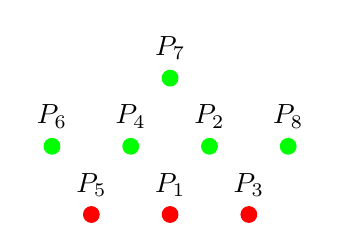
\begin{tikzpicture}
\node[draw,circle,inner sep=2pt,fill,red,label={$P_5$}] at (-1,0) {};
\node[draw,circle,inner sep=2pt,fill,red,label={$P_1$}] at (0,0) {};
\node[draw,circle,inner sep=2pt,fill,red,label={$P_3$}] at (1,0) {};
\node[draw,circle,inner sep=2pt,fill,green,label={$P_6$}] at (-1.5,0.866) {};
\node[draw,circle,inner sep=2pt,fill,green,label={$P_4$}] at (-0.5,0.866) {};
\node[draw,circle,inner sep=2pt,fill,green,label={$P_2$}] at (0.5,0.866) {};
\node[draw,circle,inner sep=2pt,fill,green,label={$P_8$}] at (1.5,0.866) {};
\node[draw,circle,inner sep=2pt,fill,green,label={$P_7$}] at (0,1.732) {};
\end{tikzpicture}
\end{center}

\noindent
\textbf{Second solution.}
We prove more generally that for fixed positive integers $k$ and $\ell$,
if the points of the plane are colored in $k$ different colors subject to the condition that if $\ell$ distinct points on a circle are the same color, then so is the center, then again all points must be the same color.

Suppose by way of contradiction that there are points of two distinct colors, say $P_1$ (colored red) and $P_2$ (colored green). Each circle centered at $P_i$ then contains at most $(k-1)\ell$ points that are not the color of $P_1$ (namely, at most $\ell$ point in each of the other $k-1$ colors). Now draw $m$ distinct circles around each $P_i$, each of radius greater than the distance $P_1P_2$; these circles meet in $2m^2$ distinct points. Of these points, at least $2m^2 - m(k-1)\ell$ are red and at least $2m^2 - m(k-1)\ell$ are green, but for $m$ sufficiently large this accounts for more than $2m^2$ points, a contradiction.

\item[B2]
\noindent
\textbf{First solution.}
By writing
\[
x_1 = \frac{\int_0^1 xf(x)\,dx}{\int_0^1 f(x)\,dx}, \qquad
x_2 = \frac{\int_0^1 xf(x)^2\,dx}{\int_0^1 f(x)^2\,dx},
\]
we se that it suffices to show that $I_1<I_2$ for
\begin{align*}
I_1 &:= \left(\int_0^1 xf(x)\,dx\right)\left(\int_0^1 f(x)^2\,dx\right), \\
I_2 &:= \left(\int_0^1 f(x)\,dx\right)\left(\int_0^1 xf(x)^2\,dx\right).
\end{align*}
By Fubini's theorem, we can write each of $I_1$ and $I_2$ in terms of double integrals:
\begin{align*} I_1 &= \iint_{[0,1]^2} xf(x)f(y)^2\,dy\,dx = \iint_{[0,1]^2} yf(y)f(x)^2\,dy\,dx \\
I_2  &=\iint_{[0,1]^2} f(x)yf(y)^2\,dy\,dx = \iint_{[0,1]^2} f(y)xf(x)^2\,dy\,dx,
\end{align*}
where in each case the second double integral is obtained from the first by switching the roles of $x$ and $y$. By adding the two expressions for $I_2$ and subtracting the two expressions for $I_1$, we find that
\[
2(I_2-I_1) = \iint_{[0,1]^2} f(x)f(y)(y-x)(f(y)-f(x))\,dy\,dx.
\]
But since $f$ is strictly increasing, $(y-x)(f(y)-f(x)) \geq 0$ for all $x,y$, with equality only if $x=y$. We conclude that this final double integral is positive and thus that $I_1<I_2$, as desired.

\noindent
\textbf{Second solution.}
Let $S_1$ be the region in $\RR^3$ defined by the inequalities
\[
0 \leq x \leq 1, \, 0 \leq y \leq f(x), \, 0 \leq z \leq f(x_1).
\]
This is a prism on the base $R$, so its centroid projects to the centroid of $R$.
In particular, the centroid of $S_1$ has $x$-coordinate $x_1$.

Let $S_2$ be the region obtained from $S_1$ by removing the subset
\[
0 \leq x < x_1, \, 0 \leq y \leq f(x), \, f(x) < z \leq f(x_1)
\]
and adding the subset
\[
x_1 < x \leq 1, \, 0 \leq y \leq f(x), \, f(x_1) < z \leq f(x).
\]
Since we removed a region of positive volume to the left of the plane $x=x_1$ and added a region of positive volume to the right of it,
the centroid of $S_2$ has $x$-coordinate strictly greater than $x_1$.

Now note that $S_2$ can be described as
\[
0 \leq x \leq 1, \, 0 \leq y \leq f(x), \, 0 \leq z \leq f(x).
\]
Each cross-section of $S_2$ parallel to the $yz$ plane is a square with area $1/\pi$ times the area
of the corresponding cross-section of the solid obtained by rotating $R$ around the $x$-axis.
Consequently, the $x$-coordinate of the centroid of $S_2$ is the same as that of the solid of revolution, which is $x_2$. This shows that $x_1 < x_2$.

\item[B3]
Yes, $S$ must contain all positive integers.

\noindent
\textbf{First solution.}

We prove that $n \in S$ by strong induction on $n$. We have $1 \in S$ because $S$ is nonempty and 1 divides $2025^n-15^n$ for every $n \in S$. Now suppose that $n > 1$ and $1,\dots,n-1 \in S$.
Write $n = 3^a 5^b d$ with $a,b\geq 0$ and $\gcd(15,d)=1$, and define $c = \max(a,b)$.
Since  $d$ is coprime to $135$, we have $135^k \equiv 1 \pmod{d}$ for any $k$ divisible by $\phi(d)$ (writing $\phi$ for the Euler totient function). If $c>0$, then $(3^c-1)d > cd \geq c$, yielding
\[
\phi(d) \leq d < 3^c d - c \leq n-c
\]
and so $c < n - \phi(d)$; the same holds for $c=0$ because $\phi(d) \leq \phi(n) < n$ for $n>1$. Consequently, for
\[
k := \phi(d) \lfloor (n-1)/\phi(d) \rfloor > n-1-\phi(d) \geq c,
\]
$n$ divides $15^k (135^k-1) = 2025^k - 15^k$ and so $n \in S$.

\noindent
\textbf{Second solution.} (suggested by Evan Dummit)
Define the sequence $\{a_i\}$ by 
\[
a_0 = 1, a_{i+1} = 2025^{a_i} - 15^{a_i} \quad (i \geq 0).
\]
By induction on $i$, $a_i$ divides $a_{i+1}$: this is obvious for $i=0$, while for the induction step we apply the identity
\[
x^{md}-y^{md} = (x^m-y^m)(x^{m(d-1)} + \cdots + y^{m(d-1)})
\]
to see that if $a_i$ divides $a_{i+1}$, then $2025^{a_i}-15^{a_i}$ divides $2025^{a_{i+1}}-15^{a_{i+1}}$.

We prove that every positive integer divides some $a_i$. Suppose by way of contradiction that this fails, and let $n$ be the smallest positive integer not dividing any $a_i$. This $n$ cannot equal $1$.
Let $p$ be the smallest prime factor of $n$, and write $n = p^e m$ with $m$ coprime to $p$;
then $m < n$ and so $m$ divides some $a_i$, and hence every subsequent $a_i$ (by the previous paragraph). If $p^e < n$ then $p^e$ also divides all sufficiently large $a_i$, as then does $\mathrm{lcm}(p^e, m) = n$, a contradiction; hence $n = p^e$ is a prime power. We cannot have $p=3$ or $p=5$ because the $a_i$ tend to $\infty$ and $a_{i+1}$ is divisible by $15^{a_i}$; hence $n$ is coprime to $135$.
Since $\phi(n) < n$, $\phi(n)$ must divide some $a_i$; but now $n$ divides $135^{a_i}-1$ and hence also $a_{i+1}$, again a contradiction.

\item[B4]
\noindent
\textbf{First solution.}
For $i,j \in \{1,\dots,n\}$, define
\[
d_{i,j} = \min\{|i-i'|+|j-j'|\colon a_{i',j'} = 0\};
\]
this measures the distance from $(i,j)$ to the set of $(i',j')$ where $a_{i',j'}=0$ in the \emph{taxicab metric}.
It follows from conditions (b) and (c) that $a_{i,j} \leq d_{i,j}$; moreover, $d_{i,j}$ also satisfies conditions (a)--(c) with the same value of $N$. Consequently, it is sufficient to prove
$S \leq (n+2)N/3$ when $a_{i,j} = d_{i,j}$ for all $i,j$, i.e., when $A$ is a \emph{taxicab matrix}
in addition to satisfying (a)--(c). We will prove this by induction on $n$,
checking the base case $n=2$ by verifying that $S \leq (n+2)N/3$ when $A$ is one of
\[
\begin{pmatrix} 0 & 0 \\
0 & 0 \end{pmatrix},
\begin{pmatrix} 0 & 0 \\
0 & 1 \end{pmatrix},
\begin{pmatrix} 0 & 0 \\
1 & 1 \end{pmatrix},
\begin{pmatrix} 0 & 1 \\
0 & 1 \end{pmatrix},
\begin{pmatrix} 0 & 1 \\
1 & 2 \end{pmatrix}.
\]
Alternatively, one can extend the problem to $n=1$ by specifying that in that case $a_{1,1} \in \{0,1\}$, and then the induction step will also cover $n=2$.

Let $c_k$ denote the number of entries of $A$ equal to $k$.
We next prove that $c_k > c_{k+1}$ for any $k>0$ with $c_k > 0$,
by showing that the following recipe defines
an injective but not surjective map from pairs $(i,j)$ with $a_{i,j}=k+1$
to pairs $(i,j)$ with $a_{i,j} = k$: map $(i,j)$ to $(i-1,j)$ if $a_{i-1,j} = k$ and to $(i-1,j-1)$ otherwise. To confirm that this map is well-defined, injective, and not surjective, we must check four points.
\begin{itemize}
\item
The assigned value belongs to $\{1,\dots,n\} \times \{1,\dots,n\}$. 
This is only an issue when $i=1$ or $j=1$, but in those cases conditions (a)--(c) imply that $a_{i,j} \leq 1$. Consequently, we cannot have $a_{i,j} = k+1$ for $k>0$.
\item
The assigned value $(i',j')$ satisfies $a_{i',j'} = k$. This is clear when $(i',j') = (i-1,j)$.
Otherwise, we have $a_{i-1,j} = k+1$ and $(i',j') = (i-1,j-1)$. 
Now comparing with $a_{i,j}$ shows that $a_{i,j-1} \in \{k,k+1\}$, but $a_{i,j-1} =k+1$ would force $a_{i,j} = k+2$ because $A$ is a taxicab matrix;
hence $a_{i,j-1} = k$.
Finally, comparing with $a_{i-1,j}$ and $a_{i,j-1}$ shows that $a_{i-1,j-1} = k$.
\item
No value $(i,j)$ with $a_{i,j} = k$ can occur as the image of both $(i+1,j)$ and $(i+1,j+1)$.
This would imply firstly $a_{i+1,j} = k+1$ and secondly $a_{i,j+1} = a_{i+1,j+1} = k+1$, but these cannot both hold: because $A$ is a taxicab matrix, $a_{i+1,j} = a_{i,j+1} = k+1$ would force $a_{i+1,j+1} = k+2$.
\item
There is a value $(i,j)$ with $a_{i,j}=k$ that is not assigned. 
To wit, every row containing $k+1$ also contains $k$; so for the largest $i$ for which $a_{i,j} = k+1$ for some $j$, then there also exists $j$ such that $a_{i,j} = k$ and the pair $(i,j)$ cannot be assigned.
\end{itemize}

Returning to the induction step, subtracting 1 from all nonzero entries and deleting the first row and column yields another taxicab matrix. As this operation replaces $S, N, n$ with $S-N, N-c_1, n-1$ respectively, the induction hypothesis implies that
\[
S-N \leq \frac{n+1}{3}(N-c_1),
\]
and so it will suffice to prove that 
\[
N \leq \frac{N-c_1}{3} + \frac{n+2}{3}c_1 \Longleftrightarrow 2N \leq (n+1)c_1.
\]
This is apparent if $c_1 \geq n$ because $N \leq \tfrac{n(n+1)}{2}$.
Otherwise, the nonzero values of $c_k$ form a strictly decreasing sequence starting with $c_1$ and summing to $N$, and so
\[
N \leq \frac{c_1(c_1+1)}{2} \leq \frac{(n+1)c_1}{2}.
\]

\noindent
\textbf{Second solution.}
(Art of Problem Solving, user hliu1)
Let $B$ (resp.\ $C$)
be the matrix obtained from $A$ by reversing the nonzero entries in each row (resp. column),
keeping the zero entries in the same positions. Since the entries of $B$ and $C$ are permutations of the entries of $A$, the sum of entries of $A+B+C$ equals $3S$.

Since $a_{i,j} = 0$ when $i+j \leq n$
and $a_{i,j+1}, a_{i+1,j} \leq a_{i,j}+1$,
by induction on $i+j$ we obtain
\[
a_{i,j} \neq 0 \Longrightarrow a_{i,j} \leq i+j-n.
\]
Next, note that the first nonzero entry in each row of $A$ is 1, so $b_{i,n} \leq 1$.
Since $b_{i,j} \leq b_{i,j+1}+1$ for $j < n$,
\[
a_{i,j} \neq 0 \Longrightarrow b_{i,j} \leq n+1-j.
\]
By similar logic with the rows and columns reversed,
\[
a_{i,j} \neq 0 \Longrightarrow c_{i,j} \leq n + 1 - i.
\]
Summing yields
\[
a_{i,j} \neq 0 \Longrightarrow a_{i,j} + b_{i,j} + c_{i,j} \leq n+2.
\]
Now summing over the nonzero entries of $A+B+C$ yields $3S \leq (n+2) N$ as desired.

\noindent
\textbf{Remark.}
The second solution gives rise to an analogous statement about $k$-dimensional arrays of nonnegative integers for any $k$.

\item[B5]
Let $f(p)$ denote the number of $k \in \{1,\dots,p-2\}$ such that $I(k+1) < I(k)$.
We prove that $f(p) > \tfrac{p}{4}-1$ for $p > 3$ by deriving an exact formula for $f(p)$.

In the field $\mathbb{F}_p$ we have the identity
\[
\frac{1}{k+1} + \frac{1}{1/k + 1} = 1 \qquad (k \neq -1).
\]
This implies that for $k=1, \dots, p-2$,
\[
I(k+1) + I(I(k)+1) = p+1:
\]
the left-hand side is congruent to 1 modulo $p$, but each summand is in $\{1,\dots,p-1\}$
so the sum lies strictly between $1$ and $2p+1$.

Since we cannot have $I(k+1) = I(k)$, we can interpret $f(p)$ as the number of $k \in \{1,\dots,p-2\}$ such that $I(k+1) < I(k)+1$, or equivalently
\[
I(k)+1 + I(I(k)+1) > p+1.
\]
Set $m := I(k)+1$; as $k$ runs over $\{1,\dots,p-2\}$, $I(k)$ also runs over $\{1,\dots,p-2\}$
(because $I(p-1) = p-1$) and so $m$ runs over $\{2,\dots,p-1\}$. 
Consequently, $f(p)$ counts
$m \in \{2,\dots,p-1\}$ such that
\[
m + I(m) > p+1,
\]
or equivalently $m \in \{1,\dots,p-1\}$ since $m=1$ never satisfies the condition.

By writing $I(p-m) = p-I(m)$, we see that
\[
p-m + I(p-m) = 2p - (m + I(m)).
\]
Consequently, exactly one of $m+I(m) > p+1$ or $p-m+I(p-m) > p+1$ holds unless
$m+I(m) \in \{p-1, p, p+1\}$. By symmetry, $f(p)$ equals $\frac{p-1}{2}$ minus half the number of $m \in \{1,\dots,p-1\}$ with $m+I(m) \in \{p-1, p, p+1\}$.

Since $p > 3$, $m+I(m) = p\pm 1$ if and only if $m^2 \pm m + 1 = 0$ in $\mathbb{F}_p$;
for each sign, we get 2 solutions if $p \equiv 1 \pmod{3}$ and 0 otherwise. Similarly, $m+I(m) = p$ if and only if $m^2+1 = 0$ in $\mathbb{F}_p$; we get 2 solutions if $p \equiv 1 \pmod{4}$ and 0 otherwise. Hence $f(p)$ equals
\[
\frac{p-1}{2} - (2 \text{ if } p \equiv 1 \!\!\!\!\!\!\pmod{3}) - (1 \text{ if } p \equiv 1 \!\!\!\!\!\!\pmod{4}).
\]
In particular, $f(p) - \left(\tfrac{p}{4} -1\right)\geq \tfrac{p-1}{2} - 2 - \tfrac{p}{4} = \tfrac{p-10}{4}$.
This proves the claim for $p \geq 11$; for $p=5,7$ we compute directly that $f(p) = 1 > \tfrac{p}{4}-1$.

\item[B6]
The largest such constant is $r=\tfrac{1}{4}$. This value works because we may take $g(n) = n^2$.

By way of contradiction, suppose such a function $g$ exists for some $r > \tfrac{1}{4}$.
Since $g$ takes positive integer values, $g(n+1) - g(n) > g(g(n))^r > 0$ for all $n$.

We next note that for $s \in [0, \infty)$ the minimum of $rs^2 + 1 - s$
is $1-\tfrac{1}{4r}> 0$ (achieved at $s = \tfrac{1}{2r}$), so the sequence
\[
s_0 = 0, \qquad s_{n+1} = rs_n^2 + 1
\]
is strictly increasing and unbounded.

In the following arguments, we make a number of statements over positive integers $n$ and an auxiliary real parameter $s \geq 0$. For notational convenience, we adopt the convention that $*$ always represents a positive constant dependent on $s$ but not $n$, but \emph{no two} appearances of $*$ necessarily represent the \emph{same} positive constant.

We next prove that for any $s \geq 0$, we have $g(n) \geq n^s$ for $n \geq *$.
This is evident for $s=0$; since the sequence $\{s_n\}$ is unbounded, it is sufficient to ``induct''
by deducing that the claim for some $s$ implies the same for $rs^2+1-\epsilon$ for any $\epsilon > 0$. To wit,
if $g(n) \geq * n^s$ for $n \geq *$, then by telescoping and monotonicity, for $n \geq *$ we have
\begin{align*}
g(n) &\geq \sum_{m=*}^{n-1} g(g(m))^r \geq \sum_{m=*}^{n-1} g(\lfloor * m^{s}\rfloor )^r \\
&\geq \sum_{m=*}^{n-1} (* m^{s^2})^r \geq * n^{rs^2+1} \geq n^{rs^2+1-\epsilon}.
\end{align*}

Applying the previous paragraph for some $s > 4$, for $n \geq *$ we obtain
\begin{align*}
g(n) &> g(n)-g(n-1) \geq g(g(n-1))^r \\
&> g((n-1)^s)^r > g(n^4)^{1/4}
\end{align*}
and thus $g(n^4) < g(n)^4$. 
Fix some $n \geq *$ and choose $M$ for which $g(n) < n^M$;
we can then induct on $k$ to obtain $g(n^{4^k}) < (n^{4^k})^M$,
contracting the previous paragraph.

\noindent
\textbf{Remark.}
There are numerous paths from the bound $g(n) \geq n^s$ to the final contradiction.
We give one alternative here: for some $s > 16$, for $n \geq *$ we have
\begin{align*}
g(n) &> g(n) - g(n-1) \geq g(g(n-1))^r \\
&\geq g(n-1)^{rs} \geq g(n-1)^{4s-1} g(n-1) \\
&\geq 3 g(n-1),
\end{align*}
yielding $g(n) > 2^n$ and hence (still for $n \geq *$)
\begin{align*}
g(n) &> g(n)-g(n-1) \geq g(g(n-1))^r \\
&\geq g(2^n)^r \geq g(2^n-1)^{r^2s} \\
&\geq g(2^{n-1})^{16s-1} g(2^{n-1}) \\
&> 2g(2^{n-1}-1) \geq 2g(n),
\end{align*}
a contradiction.


\end{itemize}
\end{document}



